\documentclass[12pt]{article}
\usepackage[utf8]{inputenc}
\usepackage{graphicx}
\usepackage[left=2.5cm,right=2cm,top=2cm,bottom=2cm]{geometry}
\usepackage{setspace}
\onehalfspacing
\usepackage{fancyhdr}

\pagestyle{fancy}
\fancyhf{}
\rhead{\textit{Stamurean Patrick Ioan}}
\lhead{Universitatea Politehnica Timișoara}
\chead{CTI-RO}
\rfoot{\centering{\thepage}}

\title{\uppercase{\bfseries{Sistem bazat pe AMD ZYNQ 7000 pentru validarea unui sistem de procesare de tip streaming cu interfata AXI stream}}}
\author{Candidat: Stamurean Patrick Ioan\\Coordonator științific: Profesor dr. ing. Oana Americai-Boncalo}
\date{Sesiunea: Iunie 2024}



\begin{document}
%%%%%%%%%% Titlu %%%%%%%%%%
\maketitle



%%%%%%%%%% Cuprins %%%%%%%%%%
\newpage
\renewcommand{\contentsname}{Cuprins}
\tableofcontents



%%%%%%%%%% Introducere %%%%%%%%%%
\newpage
\section{\uppercase{Introducere}}
\subsection{Specificatie}
Obiectivul principal al lucrării este de a proiecta și valida un sistem de procesare de tip streaming bazat pe platforma AMD ZYNQ 7000, care să permită manipularea eficientă a fluxurilor de date în timp real printr-o interfață AXI Stream. Sistemul va integra funcționalități cheie în FPGA, inclusiv gestionarea stărilor (hold, soft reset), marcarea temporală (timestamp), supraveghere (watchdog), și programare prin AXI Lite, alături de logica opțională pentru integrare, cum ar fi FIFO de intrare și ieșire. În plus, software-ul încorporat pe procesorul dual-core ARM va calcula modelul C pentru blocurile de construcție ale procesării streaming, în timp ce modulele DMA vor facilita intrarea și ieșirea datelor. Această lucrare va utiliza software-ul Vivado + Vitis pentru dezvoltare și va fi implementată pe hardware-ul ARM ZYNQ, urmărind un design de referință specificat.\\\\
Pentru proiectul bazat pe sistemul AMD ZYNQ 7000 destinat validării unui sistem de procesare de tip streaming cu interfața AXI stream, componentele principale și interfețele folosite, inclusiv lățimea de bandă (în biți), pot fi descrise astfel:

\subsubsection{Componente ale Sistemului}
\textbf{ZYNQ Processing System (PS):} Nucleul sistemului care combină capabilități de procesare pe un procesor dual-core ARM Cortex-A9 împreună cu logica programabilă FPGA.\\
\textbf{Block RAM (BRAM):} Memorie volatilă utilizată pentru stocarea temporară a datelor în FPGA.\\
\textbf{First-In, First-Out (FIFO) Buffers:} Folosite pentru a gestiona fluxul de date între diferite părți ale sistemului, asigurând o comunicare eficientă fără pierderi de date.\\
\textbf{General-Purpose Input/Output (GPIO):} Utilizate pentru soft reset și funcționalitatea de hold.\\
\textbf{Timer:} Pentru a marca evenimente temporale și pentru funcționalități de timeout.\\
\textbf{Watchdog Timer:} Asigură că sistemul răspunde în mod adecvat la erori sau blocaje, resetand sistemul dacă este necesar.\\
\textbf{AXI Interconnect:} Facilitează comunicația între diferite blocuri IP în cadrul FPGA, utilizând protocolul AXI pentru a interconecta PS cu logică programabilă și alte periferice.\\
\textbf{AXI Direct Memory Access (DMA):} Permite transferul rapid de date între memoria sistemului și FPGA, minimizând întârzierile și încărcarea procesorului.\\

\subsubsection{Interfețele Folosite}
\textbf{AXI Stream Interface:} Folosit pentru transferul de date în timp real în și din FPGA. Lățimea de bandă este variabilă, adaptată la cerințele specificului de proiect.\\
\textbf{AXI Lite Interface:} Utilizat pentru programarea și controlul configurării blocurilor IP din FPGA. De obicei, este pe 32 de biți.\\

\subsubsection{Conectivitate și Configurație}
\textbf{FPGA și PS} sunt interconectate prin AXI Interconnect, permițând un schimb eficient de date și comenzi între logica programabilă și procesor.\\
\textbf{BRAM și FIFO} sunt conectate la fluxurile de date necesare prin AXI Stream, gestionand temporizarea și bufferizarea datelor.\\
\textbf{GPIO, Timer,} și \textbf{Watchdog} sunt configurate prin AXI Lite, permitând un control fin al funcționalităților de bază și a mecanismelor de siguranță.\\
\textbf{DMA} este configurat să faciliteze transferurile eficiente de date între memoria sistemului și periferice, utilizând interfața AXI Stream pentru transferul de date și AXI Lite pentru controlul și configurarea DMA.\\
Prin această arhitectură, sistemul oferă o platformă robustă și flexibilă pentru procesarea streaming.\\
Într-un sistem bazat pe AMD ZYNQ 7000 care implementează un sistem de procesare de tip streaming cu interfață AXI stream, responsabilitățile și operațiunile sunt împărțite între software-ul rulat pe procesorul dual-core ARM (Software, sau SW) și logica programabilă FPGA. Această diviziune exploatează forțele fiecărei componente pentru a maximiza performanța și eficiența sistemului.\\

\subsubsection{Ce execută Software-ul (pe procesorul ARM)}
\textbf{Calculul Modelului C:} Software-ul implementează modelul de calcul C pentru blocurile de construcție ale procesării streaming. Aceasta înseamnă executarea algoritmilor specifici aplicației care procesează datele de intrare într-o manieră secvențială sau bazată pe evenimente.\\
\textbf{Multithreading:} Exploatează capabilitățile dual-core ale procesorului ARM pentru a rula sarcini în paralel. Aceasta poate include procesarea datelor de intrare, gestionarea comunicațiilor de rețea sau interacțiunea cu utilizatorul.\\
\textbf{Suport pentru Întreruperi:} Gestionarea întreruperilor hardware pentru a răspunde rapid la evenimente externe sau interne, cum ar fi finalizarea transferurilor DMA, semnale de la periferice sau timeri expirați.\\
\textbf{Configurarea și Controlul DMA:} Inițializarea și configurarea transferurilor DMA pentru a optimiza transferul de date între memoria sistemului și FPGA, reducând astfel sarcina procesorului și întârzierile.\\

\subsubsection{Ce execută FPGA}
\textbf{Funcționalități Cheie:} Implementează funcționalități specifice aplicației, cum ar fi hold, soft reset, timestamping și watchdog, care sunt esențiale pentru gestionarea stării sistemului și a datelor.\\
\textbf{Logica de Integrare:} Include FIFO de intrare și ieșire pentru bufferizarea datelor, logica calculată de software pentru prelucrarea datelor de ieșire.\\
\textbf{Procesarea Datelor Streaming:} Realizează prelucrarea de bază și filtrarea datelor de intrare în timp real, utilizând capacitățile de procesare paralelă ale FPGA-ului. Acest lucru este crucial pentru aplicațiile care necesită prelucrarea rapidă a volumelor mari de date, cum ar fi procesarea semnalului sau a imaginii.\\
\textbf{Comunicarea prin AXI Stream:} Generează transferul de date în timp real în cadrul sistemului, folosind interfețe AXI Stream pentru a conecta diferite blocuri de procesare și memorie în FPGA.\\\\
Cerințele de cost și throughput pentru un sistem de procesare de tip streaming bazat pe platforma AMD ZYNQ 7000 depind foarte mult de specificul aplicației și de design-ul sistemului. Totuși, putem discuta în termeni generali despre cerințele pentru modurile de operare diferite, cum ar fi \textbf{single frame, multiple frame} și \textbf{multiple frame cu repeat,} privind capacitatea sistemului de a procesa un anumit număr de biți pe secundă.\\\\

\textbf{Single Frame Mode}
În modul single frame, sistemul procesează un singur cadru de date la un moment dat. Throughput-ul necesar va depinde de mărimea cadrelor și de rata la care acestea trebuie procesate. De exemplu, dacă un cadru este de 1 MB (megabyte) și cerința este de a procesa 30 de cadre pe secundă (fps), throughput-ul necesar va fi:
\\\\Throughput = Marimea Cadru × Rate Cadre = 1 MB × 30 = 30 MB/s\\\\
Conversia în biți: 30 MB/s × 8 = 240 Mbps\\

\textbf{Multiple Frame Mode}
În modul multiple frame, sistemul procesează mai multe cadre simultan. Acest lucru necesită un throughput semnificativ mai mare, deoarece capacitatea sistemului trebuie să suporte sumarea ratelor de procesare pentru fiecare cadru individual. Dacă sistemul ar trebui să proceseze, de exemplu, 3 fluxuri diferite la 30 fps fiecare, cu aceeași mărime a cadrelor de 1 MB, throughput-ul necesar ar fi triplat:
Throughput = 3 × 240 Mbps = 720 Mbps\\\\

\textbf{Multiple Frame Mode cu Repeat}
Modul multiple frame cu repeat presupune re-procesarea aceluiași set de cadre multiple ori. Dacă fiecare cadru trebuie repetat de două ori înainte de procesarea următorului set, atunci throughput-ul necesar se dublează față de cel calculat pentru multiple frame mode:
Throughput = 720 Mbps × 2 = 1440 Mbps

\subsubsection{Considerații de Cost}
\textbf{Costul Hardware:} Capacitatea de throughput mai mare necesită hardware mai performant, care poate crește costul sistemului. FPGA-urile mai avansate și cu o capacitate mai mare de procesare sunt, de obicei, mai scumpe.\\
\textbf{Costul Dezvoltării:} Implementarea logicii necesare pentru a suporta throughput-uri mari poate fi mai complexă și necesită mai mult timp și resurse, ceea ce, de asemenea, influențează costul total al proiectului.\\\\
În contextul unui sistem bazat pe AMD ZYNQ 7000 destinat validării unui sistem de procesare de tip streaming cu interfață AXI stream, programabilitatea prin software se referă la capacitatea de a configura, controla și modifica funcționarea hardware-ului și a logicii sistemului fără a fi necesare modificări fizice ale hardware-ului. Aceasta include o gamă largă de funcționalități, de la configurarea parametrilor de sistem până la actualizarea algoritmilor de procesare.

\subsubsection{Programarea și Controlul FPGA}
\textbf{Configurarea IP-urilor FPGA:} Parametrii blocurilor de proprietate intelectuală (IP) în FPGA, cum ar fi BRAM, FIFO, GPIO, TIMER, WATCHDOG, INTERCONNECT, și AXI DMA, pot fi configurați prin software pentru a îndeplini cerințe specifice de procesare, timing sau comunicație.\\
\textbf{Actualizarea Logicii de Aplicație:} Logica specifică aplicației implementată în FPGA poate fi modificată sau actualizată prin reconfigurarea FPGA-ului cu un nou bitstream, permițând îmbunătățirea performanței sau adăugarea de noi caracteristici.\\\\\\\\

\subsubsection{Programarea Procesorului ARM}
\textbf{Multithreading și Gestionarea Întreruperilor:} Software-ul poate implementa și gestiona thread-uri multiple pentru executarea concurentă a sarcinilor, precum și pentru gestionarea întreruperilor pentru a răspunde la evenimente hardware în timp real.\\
\textbf{Configurarea DMA:} Transferurile DMA pot fi configurate și gestionate pentru a optimiza fluxul de date între memoria sistemului și periferice sau FPGA, reducând sarcina de procesare pe CPU.\\

\subsubsection{Programarea Funcționalităților Specifice}
\textbf{Controlul Funcționalităților de Bază:} Funcții precum soft reset, timing, și funcționalitățile watchdog pot fi controlate prin software, oferind un mecanism flexibil pentru gestionarea stării sistemului.\\
\textbf{Configurarea Parametrilor de Procesare:} Parametrii specifici algoritmilor de procesare, cum ar fi coeficienții de filtrare sau pragurile de decizie, pot fi ajustați din software, permitând optimizări și adaptări rapide la condiții variabile de funcționare.\\\\
Prin intermediul software-ului, sistemul oferă o mare flexibilitate și capacitate de adaptare, permițând actualizări și optimizări post-dezvoltare fără necesitatea intervențiilor hardware, ceea ce este esențial pentru adaptarea la cerințele în schimbare și pentru îmbunătățirea continuă a performanței sistemului.\\\\
Urmatoarea listă reprezinta milestone-uri detaliate pentru proiectul de licență. Acest plan este sugerat pentru mai multe săptămâni, in care descomp diferitele componente ale proiectului în sarcini gestionabile.

\subsection{Plan de executie Milestone-uri}
\textbf{Săptămâna 1: Inițierea proiectului}\\
Task 1.1: Efectuați o revizuire detaliată a cerințelor și specificațiilor proiectului.\\
Task 1.2: Configurați mediul de dezvoltare: Instalați Vivado+EDK și pregătiți configurarea hardware-ului ARM ZYNQ.\\
Task 1.3: Elaborarea planului inițial al proiectului, inclusiv etapele de referință și livrabile.\\\\
\textbf{Săptămâna 2: Proiectare și planificare preliminară}\\
Task 2.1: Aprofundare în documentația AMD ZYNQ 7000 și în nucleele IP relevante (SISTEMUL DE PROCESARE ZYNQ, BRAM, FIFO etc.).\\\\
\textbf{Săptămâna 3: Dezvoltarea funcționalității de bază FPGA - Partea 1}\\
Task 3.1: Începeți dezvoltarea FPGA cu funcționalități de bază: hold, soft reset și timestamp.\\
Task 3.2: Implementați funcționalitatea watchdog și interfața de bază de programare AXI Lite.\\
Task 3.3: Efectuați testarea inițială a funcționalităților FPGA implementate.\\\\
\textbf{Săptămâna 4: Dezvoltarea funcționalității de bază FPGA - Partea 2}\\
Task 4.1: Dezvoltați FIFO de intrare și FIFO de ieșire pentru fluxul de date.\\
Task 4.2: Efectuați testarea inițială a funcționalităților FPGA implementate.\\\\
\textbf{Săptămâna 5: Configurare DMA și integrare software}\\
Task 5.1: Configurați DMA pentru fluxul de intrare și de ieșire.\\
Task 5.2: Începeți integrarea funcționalităților FPGA cu software-ul încorporat.\\\\
\textbf{Săptămâna 6: Integrarea sistemului și testarea inițială}\\
Task 6.1: Integrați toate funcționalitățile FPGA dezvoltate.\\
Task 6.2: Efectuați testarea integrării la nivel de sistem.\\\\
\textbf{Săptămâna 7 - 8 - 9 - 10: Dezvoltare software încorporat - Configurare inițială}\\
Task 7/ 8/ 9/ 10.1: Mediul de dezvoltare a procesorului dual-core ARM.\\
Task 7/ 8/ 9/ 10.2: Dezvoltarea modelului C pentru blocurile de procesare în flux.\\
Task 7/ 8/ 9/ 10.3: Multithreading de bază și gestionarea întreruperilor în software.\\\\
\textbf{Săptămâna 11: Dezvoltare și optimizare avansată de software}\\
Task 11.1: Optimizați software-ul încorporat pentru performanță și fiabilitate.\\
Task 11.2: Îmbunătățiți software-ul cu funcții suplimentare bazate pe feedback-ul de testare a integrării.\\
Task 11.3: Implementați capabilități avansate de gestionare a întreruperilor și multithreading.\\\\
\textbf{Săptămâna 12: Testare cuprinzătoare a sistemului}\\
Task 12.1: Efectuați teste cuprinzătoare ale sistemului, inclusiv teste de stres, performanță și fiabilitate.\\
Task 12.2: Rafinați sistemul pe baza rezultatelor cuprinzătoare ale testării.\\
Task 12.3: Validați funcționalitatea finală a sistemului în raport cu cerințele inițiale.\\\\\\\\\\
\textbf{Săptămâna 13 - 14 - 15: Finalizare și documentare}\\
Task 13/ 14/ 15.1: Finalizați toate funcționalitățile sistemului și asigurați conformitatea cu specificațiile proiectului.\\
Task 13/ 14/ 15.2: Compilați documentația cuprinzătoare a proiectului, inclusiv detalii de proiectare, cod, proceduri de testare și rezultate.\\
Task 13/ 14/ 15.3: Pregătiți un manual de utilizare sau un ghid pentru sistemul dezvoltat.\\\\
\textbf{Săptămâna 16: Închiderea și prezentarea proiectului}\\
Task 16.1: Pregătiți prezentarea finală a proiectului, concentrându-se pe obiective, proces, provocări, soluții și realizări.\\
Task 16.2: Repetați prezentarea și anticipați întrebările.\\
Task 16.3: Trimiteți toate livrabilele proiectului, inclusiv codul, documentația și materialele de prezentare.\\
Task 16.4: Prezentați proiectul.\\\\



\begin{figure}[ht]
\centering
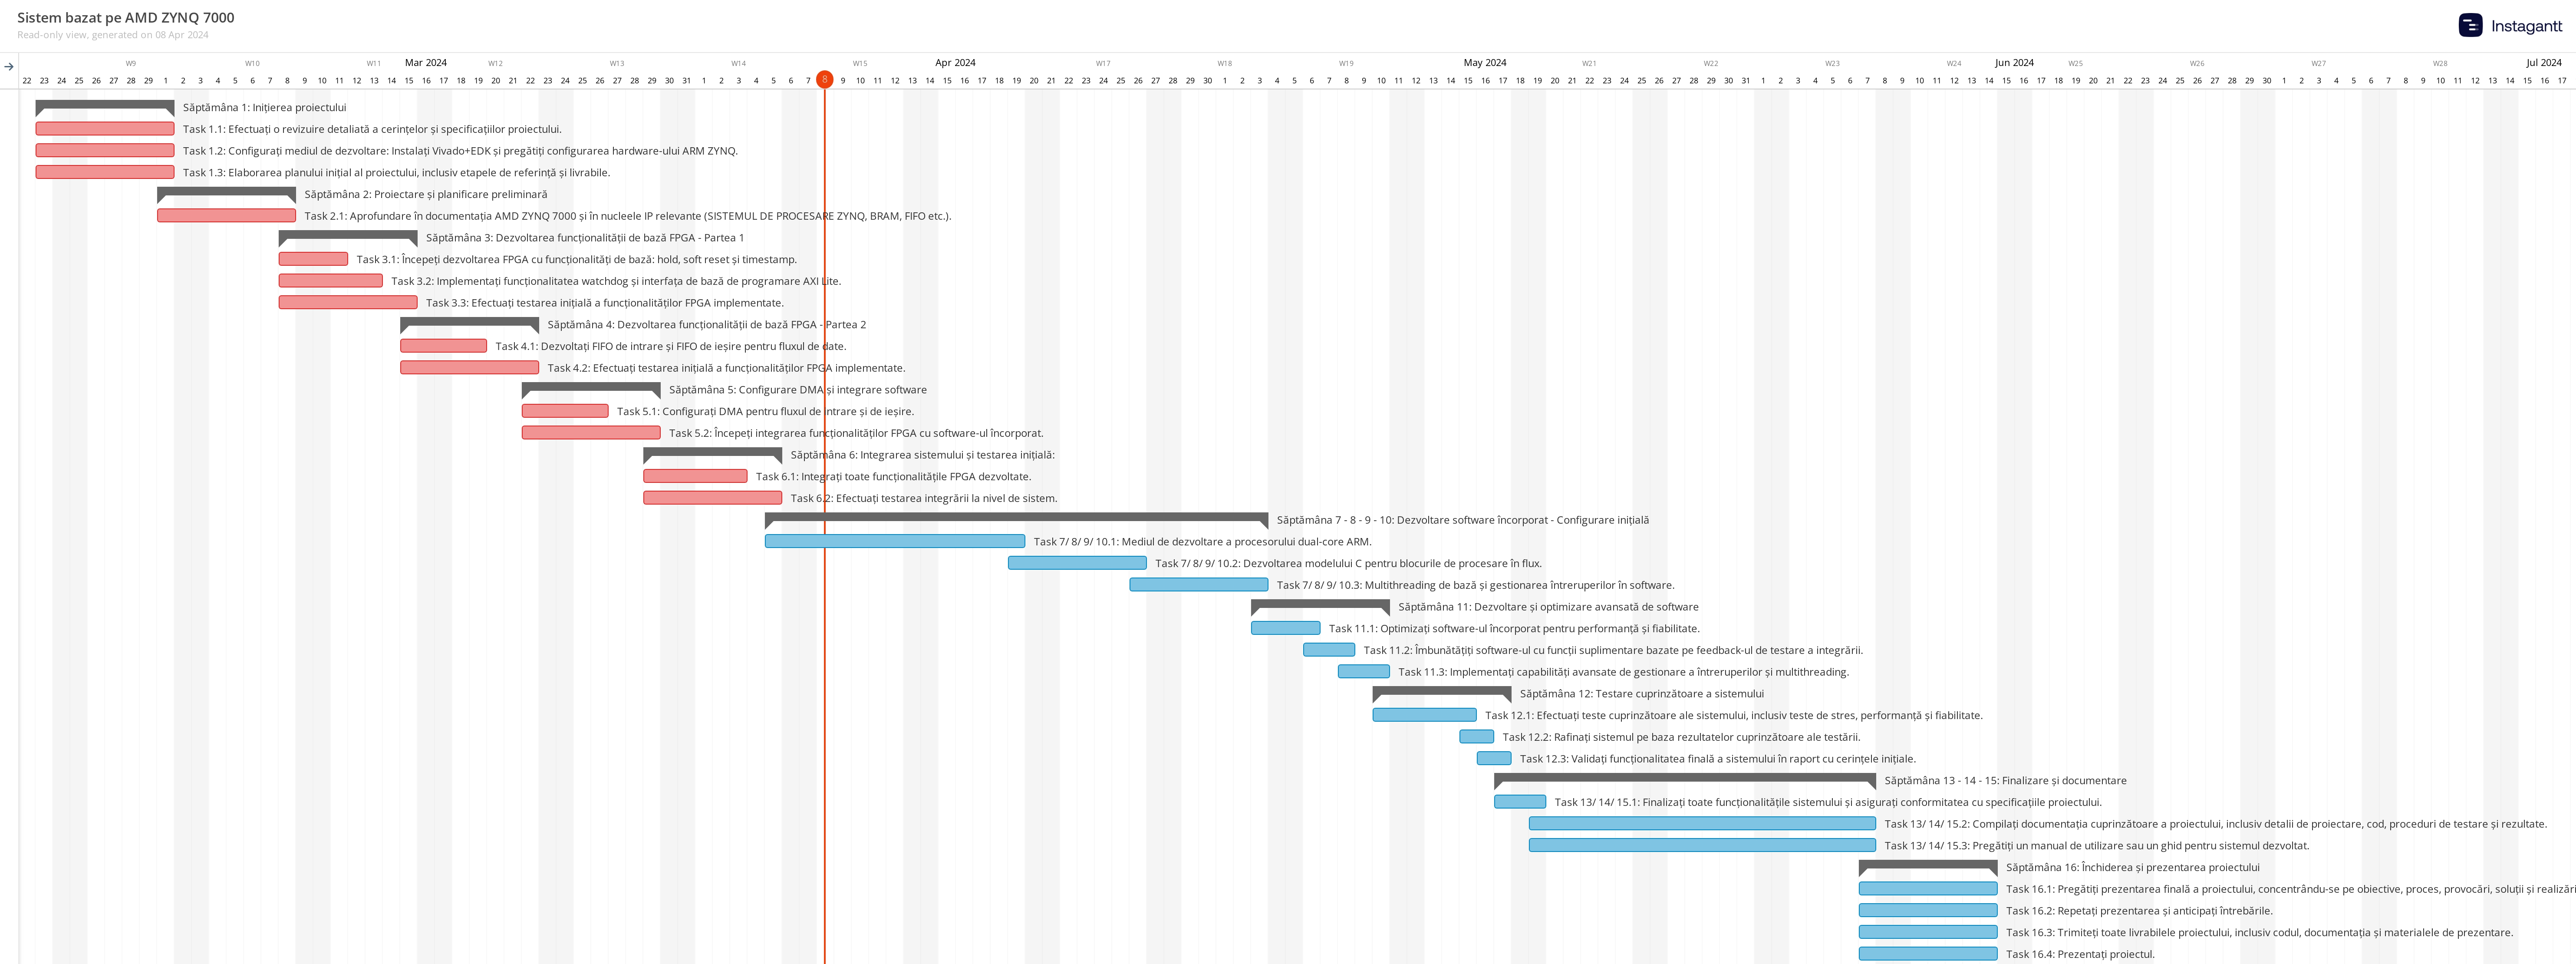
\includegraphics[width=1\textwidth]{../Licenta_Stamurean_Patrick/Milestones.jpg}
\caption{Milestones Gantt Chart \textbf{[1]}}
\end{figure}


\newpage
\section{\uppercase{Concluzii}}
Concluzii



\newpage
\begin{thebibliography}{9}
\bibitem{latexcompanion} 
Michel Goossens, Frank Mittelbach, and Alexander Samarin. 
\textit{The \LaTeX\ Companion}. 
Addison-Wesley, Reading, Massachusetts, 1993.
 
\bibitem{Gantt} 
Gantt Chart. 
\textit{https://app.instagantt.com/shared/6619061a49061f773f0c2319}. 2024.
\end{thebibliography}


\end{document}